\documentclass[11pt]{article}
\usepackage[margin=1in]{geometry}
\usepackage{amsmath,amssymb}
\usepackage{hyperref}
\usepackage{booktabs}
\usepackage{xcolor}
\usepackage{listings}
\usepackage{tikz}
\usepackage{pgfplots}
\pgfplotsset{compat=1.18}
\usetikzlibrary{positioning, arrows.meta, shapes}

\lstset{
  basicstyle=\ttfamily\footnotesize,
  breaklines=true,
  columns=fullflexible,
  showstringspaces=false,
  xleftmargin=1em,
  frame=single,
  framesep=3pt,
}

\title{Update 5-2: Architecture Comparison and RDMA's Role Per Model Family\\[4pt]
  \large Extending scuffedQuant Beyond Transformer KV Cache}
\author{Nathan Gopee\\MS Computer Science Candidate, SUNY New Paltz\\\texttt{gopeen1@newpaltz.edu}\\[4pt]Advisors: Dr.\ Wafi Danesh \& Dr.\ Ashley Suchy}
\date{April 13, 2026}

\begin{document}
\maketitle
\tableofcontents
\newpage

%==============================================================================
\section{Abstract and Recap}
%==============================================================================

Update~4 described libscuffedrdma's transport: the dual queue-pair
pool, the WFA classifier, the PMP bang-bang controller, and a
Transformer-only KV cache compressor built on
TurboQuant~\cite{zandieh2025turboquant}. Update~5 reviewed the six
upstream UCX pull requests (\#11304--\#11309) and the libmesh-rdma
hardening pass. Both are about moving bytes correctly.

Update 5-2 is about \emph{which} bytes move. Modern inference stacks
no longer draw their state from a single source: Transformer KV
caches grow linearly with context, state-space models
(Mamba-3~\cite{lahoti2026mamba3}) replace that cache with a
fixed-size hidden state, and mixture-of-experts stacks
(Granite~4~\cite{ibm2026granite4}, SonicMoE~\cite{guo2026sonicmoe})
trade both for an all-to-all expert-routing shuffle. The transport
burden is radically different in each case, and a single
`compress-then-RDMA' pipeline has to know which one it is dealing
with.

This update extends the scuffedQuant compressor to three additional
architectures (Mamba-3 SSM state, Granite~4 hybrid, and Granite~4 MoE
expert activations), introduces a shared \texttt{benchmarks/test\_arch}
harness that runs the same per-architecture probe on Chimera
(3$\times$~RTX~3090, Ampere) and Cerberus (2$\times$~RTX~5090,
Blackwell), and frames the per-architecture transport story with a
single compositional primitive borrowed from the eml universal
operator~\cite{odrzywolek2026eml}. The core Walsh-Hadamard + codebook
+ QJL math in \texttt{scuffed\_quant.py} is unchanged: two thin
shape-handling wrappers (\texttt{compress\_ssm\_state}, \texttt{compress\_expert\_activation})
are enough to cover the new architectures.

No edit is made to Update~4 or Update~5 beyond a one-line
forward-reference footnote in Update~4 \S8 so a reader tracing the
KV-compression thread knows to continue here.

%==============================================================================
\section{Why Architecture Drives the Transport Story}
\label{sec:why_arch}
%==============================================================================

The simplest observation, and the one the rest of this update
elaborates, is that the per-token state memory of modern architectures
differs by three to four orders of magnitude (Table~\ref{tab:arch_memory}).
This is a direct consequence of the self-attention complexity
analysis in the \emph{Dive into Deep Learning}
textbook~\cite{zhang2023d2l}: self-attention has $O(n^2 d)$ compute
and $O(1)$ maximum path length per layer (every token attends to
every other), while an RNN-shaped recurrence has $O(n d^2)$ compute
and $O(n)$ path length but an $O(1)$ per-step state. State-space
models like Mamba are the modern rehabilitation of the RNN side of
that table: the associative-scan trick restores parallelism while
keeping the $O(1)$ state. Once state memory is that divergent across
families, the dominant RDMA traffic pattern follows, and with it the
correct hot/cold split in libscuffedrdma's dual QP pool.

\begin{table}[htbp]
\centering
\caption{State memory and dominant transport pattern per architecture
family. Numbers assume a 7B-class dense model and a 128k context
where applicable.}
\label{tab:arch_memory}
\begin{tabular}{l l l l l}
\toprule
Family        & State/token     & Growth w/ ctx & Dominant traffic & Hot/cold bias \\
\midrule
Transformer   & $2 \cdot n_h \cdot d_h$ bytes & $O(N)$  & KV blocks       & cold (bulk KV) \\
SSM (Mamba-3) & $d_{\text{state}} \cdot d_{\text{model}}$ bytes & $O(1)$  & small-state RPC & hot (latency) \\
MoE           & $2 \cdot k \cdot d_{\text{model}}$ bytes (top-$k$) & $O(N)$ & expert all-to-all & cold + hot split \\
Hybrid        & mix of KV and SSM & mixed  & mixed  & per-layer classifier \\
\bottomrule
\end{tabular}
\end{table}

At 128k context, a 7B dense Transformer holds roughly
$2 \cdot 32 \cdot 128 \cdot 128{,}000 \cdot 2 \approx 16$~GB of KV per
user. A Mamba-3 model of similar depth holds a fixed hidden state
that is independent of context, measured in tens of megabytes. CoPE's
``free-lunch'' context extension~\cite{li2026cope} intensifies this
gap rather than closing it: clipping RoPE frequencies lets a 4k-trained
Transformer run at 128k with no retraining, but the underlying KV
cache still grows linearly, so a system that was only moving 500~MB
per user at 4k is suddenly moving 16~GB once CoPE is turned on. Under
RDMA, the Transformer case is bandwidth-bound (the cold QP saturates
the link), and the Mamba case is latency-bound (the hot QP dominates
because each state is small and must arrive quickly for the next
selective-scan step to proceed). MoE sits in between: the popular
experts look like bulk KV (cold), the rare ones look like control-plane
messages (hot). The hybrid stack in Granite~4 needs per-layer
classification because a single forward pass contains both patterns.

\begin{figure}[htbp]
\centering
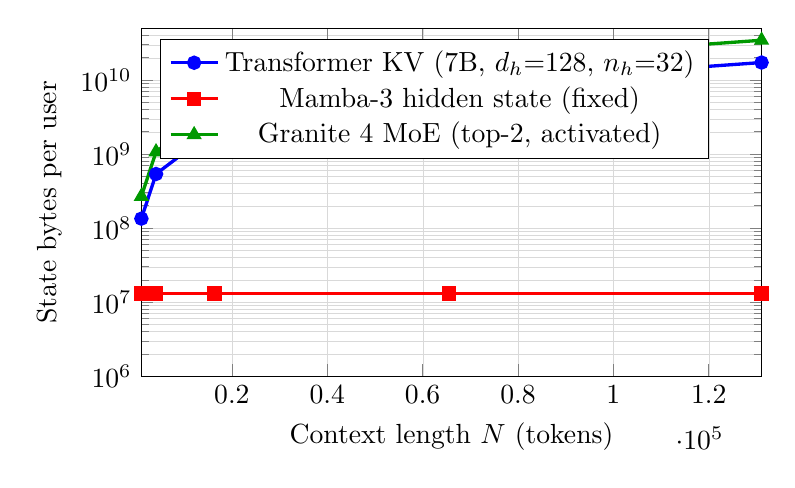
\begin{tikzpicture}
\begin{semilogyaxis}[
    width=0.78\textwidth, height=6cm,
    xlabel={Context length $N$ (tokens)},
    ylabel={State bytes per user},
    legend pos=north west,
    grid=both, grid style={line width=.1pt, draw=gray!30},
    xmin=1024, xmax=131072,
    ymin=1e6, ymax=5e10,
]
\addplot[very thick, blue, mark=*]
  coordinates {(1024,1.34e8)(4096,5.37e8)(16384,2.15e9)(65536,8.59e9)(131072,1.72e10)};
\addlegendentry{Transformer KV (7B, $d_h{=}128$, $n_h{=}32$)}
\addplot[very thick, red, mark=square*]
  coordinates {(1024,1.31e7)(4096,1.31e7)(16384,1.31e7)(65536,1.31e7)(131072,1.31e7)};
\addlegendentry{Mamba-3 hidden state (fixed)}
\addplot[very thick, green!60!black, mark=triangle*]
  coordinates {(1024,2.68e8)(4096,1.07e9)(16384,4.29e9)(65536,1.72e10)(131072,3.44e10)};
\addlegendentry{Granite 4 MoE (top-2, activated)}
\end{semilogyaxis}
\end{tikzpicture}
\caption{State bytes vs context length. Transformer KV grows linearly
with context; Mamba-3's selective-state hidden vector stays fixed;
MoE activations track the routed-token count. The four-decade gap
between the two ends of the spectrum is the transport-design story.}
\label{fig:state_vs_context}
\end{figure}

%==============================================================================
\section{Fragmentation Reloaded}
\label{sec:fragmentation}
%==============================================================================

The thesis draft's fragmentation diagram (draft1.tex, lines
762--837) is worth restating under 2026 labels. Update~4 motivated the
dual-QP architecture from the application-to-hardware fragmentation
gap below; the middleware row (NCCL, UCX, JACCL, Gloo) now has to
handle not just transport differences but architecture differences
too, because the same wire path carries very different state shapes
depending on what model is running.

\begin{figure}[htbp]
\centering
\resizebox{0.95\textwidth}{!}{%
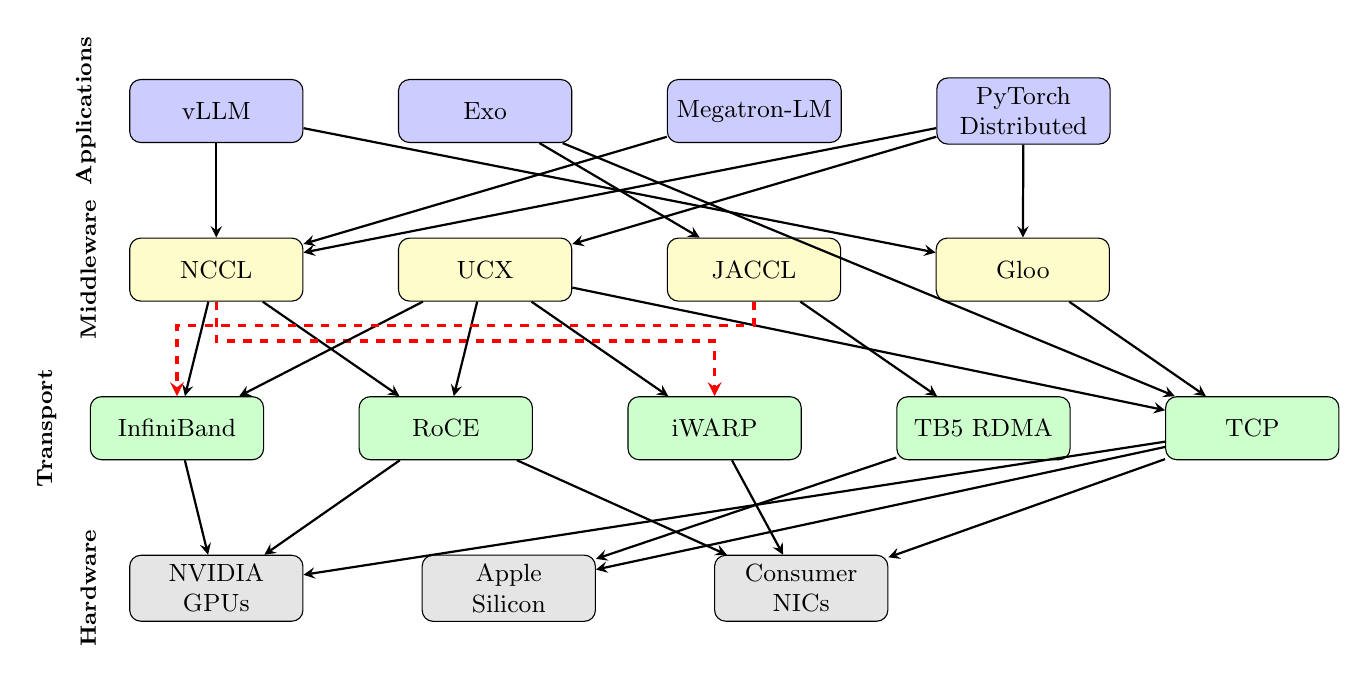
\begin{tikzpicture}[
    node distance=0.8cm and 1.2cm,
    box/.style={rectangle, draw, rounded corners, minimum width=2.2cm, minimum height=0.8cm, align=center, font=\small},
    app/.style={box, fill=blue!20},
    mid/.style={box, fill=yellow!20},
    trans/.style={box, fill=green!20},
    hw/.style={box, fill=gray!20},
    broken/.style={draw=red, very thick, dashed},
    arrow/.style={->, >=stealth, thick}
]
\node[app] (vllm) {vLLM};
\node[app, right=of vllm] (exo) {Exo};
\node[app, right=of exo] (megatron) {Megatron-LM};
\node[app, right=of megatron] (pytorch) {PyTorch\\Distributed};

\node[mid, below=1.2cm of vllm] (nccl) {NCCL};
\node[mid, right=of nccl] (ucx) {UCX};
\node[mid, right=of ucx] (jaccl) {JACCL};
\node[mid, right=of jaccl] (gloo) {Gloo};

\node[trans, below=1.2cm of nccl, xshift=-0.5cm] (ib)   {InfiniBand};
\node[trans, right=of ib] (roce)   {RoCE};
\node[trans, right=of roce] (iwarp) {iWARP};
\node[trans, right=of iwarp] (tb5)  {TB5 RDMA};
\node[trans, right=of tb5]  (tcp)   {TCP};

\node[hw, below=1.2cm of ib, xshift=0.5cm]   (nvidia)  {NVIDIA\\GPUs};
\node[hw, right=1.5cm of nvidia] (apple)   {Apple\\Silicon};
\node[hw, right=1.5cm of apple]  (consumer){Consumer\\NICs};

\draw[arrow] (vllm) -- (nccl);
\draw[arrow] (vllm) -- (gloo);
\draw[arrow] (exo) -- (jaccl);
\draw[arrow] (exo) -- (tcp);
\draw[arrow] (megatron) -- (nccl);
\draw[arrow] (pytorch) -- (nccl);
\draw[arrow] (pytorch) -- (gloo);
\draw[arrow] (pytorch) -- (ucx);

\draw[arrow] (nccl) -- (ib);
\draw[arrow] (nccl) -- (roce);
\draw[arrow, broken] (nccl.south) -- ++(0,-0.5) -| (iwarp);
\draw[arrow] (ucx) -- (ib);
\draw[arrow] (ucx) -- (roce);
\draw[arrow] (ucx) -- (iwarp);
\draw[arrow] (ucx) -- (tcp);
\draw[arrow] (jaccl) -- (tb5);
\draw[arrow, broken] (jaccl.south) -- ++(0,-0.3) -| (ib);
\draw[arrow] (gloo) -- (tcp);

\draw[arrow] (ib) -- (nvidia);
\draw[arrow] (roce) -- (nvidia);
\draw[arrow] (roce) -- (consumer);
\draw[arrow] (iwarp) -- (consumer);
\draw[arrow] (tb5) -- (apple);
\draw[arrow] (tcp) -- (nvidia);
\draw[arrow] (tcp) -- (apple);
\draw[arrow] (tcp) -- (consumer);

\node[left=0.3cm of vllm, font=\footnotesize\bfseries, rotate=90, anchor=south] {Applications};
\node[left=0.3cm of nccl, font=\footnotesize\bfseries, rotate=90, anchor=south] {Middleware};
\node[left=0.3cm of ib, font=\footnotesize\bfseries, rotate=90, anchor=south] {Transport};
\node[left=0.3cm of nvidia, font=\footnotesize\bfseries, rotate=90, anchor=south] {Hardware};
\end{tikzpicture}%
}
\caption{Fragmentation overview redrawn for 2026. The middleware row
still sees orthogonal combinations of application, transport, and
hardware, but the \emph{application} row now carries three
architecturally distinct state shapes (KV, SSM, MoE) on the same
wire.}
\label{fig:fragmentation_overview_5_2}
\end{figure}

%==============================================================================
\section{Universal Primitives: The eml Analogy}
\label{sec:eml}
%==============================================================================

Odrzyw{\'o}{\l}ek~\cite{odrzywolek2026eml} observes that a single
two-argument operator,
\[
  \mathrm{eml}(x, y) \;=\; \exp(x) - \ln(y),
\]
already contains exponentials and logarithms as special cases:
$\mathrm{eml}(x, 1) = \exp(x)$ and
$\mathrm{eml}(1, \mathrm{eml}(\mathrm{eml}(1, x), 1)) = \ln(x)$.
Two operators in one, composed from a single primitive. The analogy
for tensor transport: every architecture's per-layer traffic pattern
composes from two RDMA primitives --- \emph{classify} (WFA on a
tensor's size and access role) and \emph{allocate} (PMP on queue
occupancy). A Transformer KV block, a Mamba-3 hidden state, and a
Granite~4 expert activation are not different transport protocols;
they are different parameter choices on the same
$(\text{classify}, \text{allocate})$ pair. The next four sections
(\S\ref{sec:fa4}, \S\ref{sec:mamba3}, \S\ref{sec:moe},
\S\ref{sec:scuffedquant_ext}) spell those parameter choices out.

%==============================================================================
\section{Relative Position as a Transport Signal}
\label{sec:pos_qp}
%==============================================================================

Self-attention has no notion of token order on its own; order is
injected through positional encoding. The \emph{Dive into Deep
Learning} sinusoidal scheme~\cite{zhang2023d2l} gives each position
$i$ a vector whose coordinates are sampled from a geometric
progression of frequencies:
\[
  p_{i, 2j} \;=\; \sin\!\left(\frac{i}{10000^{2j/d}}\right),
  \qquad
  p_{i, 2j+1} \;=\; \cos\!\left(\frac{i}{10000^{2j/d}}\right).
\]
The low-frequency coordinates encode coarse position (``near the
start'' vs ``near the end'' of the context); the high-frequency
coordinates encode fine position (``three tokens ago''); relative
offsets appear as linear transforms in that space. Modern LLMs use
RoPE rather than raw sinusoidal PE, but the same frequency structure
applies: distance shows up as a rotation whose inner-product envelope
decays predictably. CoPE (Clipped RoPE)~\cite{li2026cope} is a recent
``free-lunch'' extension that clips the RoPE frequency band so a
model trained at 4k context generalises to 128k without retraining.
For our purposes CoPE \emph{strengthens} the transport prior: the
clipped spectrum sharpens the ``near vs far'' contrast at the
frequencies the classifier actually reads, so the same
$\rho_t$-based rule described below becomes more accurate under CoPE
than under vanilla RoPE. This same signal --- how far a KV entry
sits from the current decode token --- is a \emph{transport} signal,
not just a modelling signal:

\begin{itemize}
  \item \textbf{Fresh tokens} (tail of the sequence, high
  fine-frequency correlation with the current query) are read by
  attention on \emph{every} decode step. Their KV entries are
  latency-critical and small: hot QP, minimal compression.
  \item \textbf{Mid-sequence tokens} are read with decreasing
  probability as context grows. Their KV entries can travel on the
  cold QP with aggressive (3-bit) scuffedQuant; if a decode step
  does not read them, the link saved a trip.
  \item \textbf{Attention-sink tokens} (first few positions,
  well-studied in the streaming-attention literature) retain
  high attention weight regardless of distance. They should ride the
  hot QP with the freshest tokens, even though their absolute
  position index is the oldest --- proving that the correct signal
  is \emph{predicted read frequency}, not raw position.
\end{itemize}

The WFA classifier in \texttt{middleware/rdma\_tensor\_cache/wfa\_classifier.py}
currently classifies transfers by size and phase (prefill vs decode).
A natural extension, consistent with the classify--allocate
primitive in \S\ref{sec:eml}, is to add a \emph{relative-position
feature} $\rho_t = (N - t) / N$ for token $t$ in a context of length
$N$. The classifier's hot/cold decision becomes
\[
  \mathrm{hot}(t) \;=\; \big[\alpha \cdot \rho_t + \beta \cdot
  \mathbb{1}_{t \in \text{sinks}} + \gamma \cdot s_t > \tau\big],
\]
where $s_t$ is the size-class term the classifier already uses and
$\tau$ is the bang-bang threshold. Nothing about this breaks PMP:
the switching function $S$ from Update~4 still consumes the
classifier's output; it just gets a richer input. For a Transformer
at 128k context this is a one-field extension. For Mamba-3
(Section~\ref{sec:mamba3}) the feature degenerates --- there is no
per-token state to place --- and the classifier collapses back to
``always hot,'' which is the correct behaviour for an $O(1)$ state
model. For MoE (Section~\ref{sec:moe}) the same feature applies,
scored per expert rather than per token: popular experts are the
``fresh'' row, rare experts are the ``sink'' row.

The practical upshot is that the d2l.ai positional-encoding table
and libscuffedrdma's WFA classifier are computing complementary
sides of the same distribution: attention uses position to decide
\emph{which tokens to read}, and the transport layer should use
position to decide \emph{which QP to read them from}.

%==============================================================================
\section{FlashAttention-4 and Asymmetric Pipelining}
\label{sec:fa4}
%==============================================================================

FlashAttention-4~\cite{zadouri2026flashattention4} is the 2026 iteration
of Dao's attention kernel. Its central idea is explicit asymmetric
pipelining between HBM and tensor cores on Blackwell: attention
kernels stage tiles into shared memory so that tensor-core FMAs
overlap HBM loads, reaching peak arithmetic intensity without
starving the compute units.

The same asymmetry rules the RDMA layer. Our cluster has two endpoints
of very different bandwidth:
\begin{itemize}
  \item HBM on RTX~5090 (Cerberus): $\approx 800$~GB/s.
  \item 10~GbE NIC, SoftRoCE: $\approx 1.25$~GB/s.
\end{itemize}
The ratio is roughly 640$\times$. FlashAttention-4's HBM$\leftrightarrow$tensor-core
pipelining is the on-die version of what the dual QP pool does across
the NIC: the hot QP absorbs small latency-critical transfers
(analogous to register-file reads) while the cold QP carries the
bulk KV (analogous to HBM loads). Because the bandwidth gap is so
extreme, the cost of \emph{not} pipelining the two is four decades
larger on the NIC side than on the HBM side --- which is precisely
why libscuffedrdma needs an explicit split and not a single shared
CQ.

\begin{figure}[htbp]
\centering
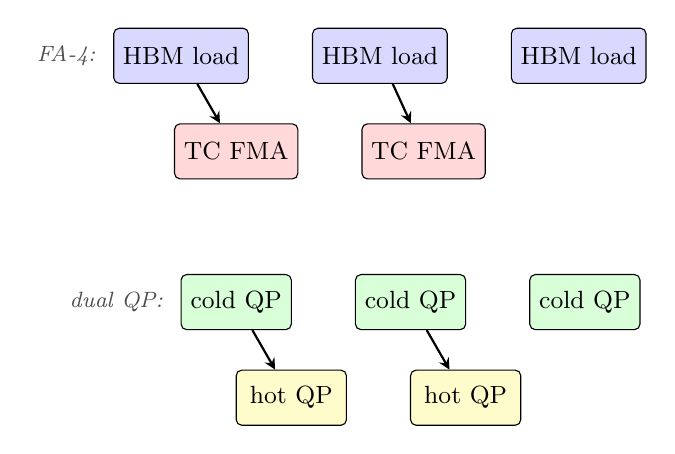
\begin{tikzpicture}[
    node distance=0.5cm and 0.8cm,
    tile/.style={draw, rounded corners=2pt, minimum height=0.7cm, minimum width=1.4cm, align=center, font=\small},
    hbm/.style={tile, fill=blue!15},
    tc/.style={tile, fill=red!15},
    nic/.style={tile, fill=green!15},
    qp/.style={tile, fill=yellow!20},
    arrow/.style={->, >=stealth, thick},
    label/.style={font=\footnotesize\itshape, text=black!70}
]
\node[hbm] (h1) {HBM load};
\node[hbm, right=of h1] (h2) {HBM load};
\node[hbm, right=of h2] (h3) {HBM load};
\node[tc, below=of h1, xshift=0.7cm] (t1) {TC FMA};
\node[tc, right=of t1] (t2) {TC FMA};

\node[label, left=0.1cm of h1] {FA-4:};
\draw[arrow] (h1) -- (t1);
\draw[arrow] (h2) -- (t2);

\node[nic, below=1.2cm of t1] (n1) {cold QP};
\node[nic, right=of n1] (n2) {cold QP};
\node[nic, right=of n2] (n3) {cold QP};
\node[qp, below=of n1, xshift=0.7cm] (q1) {hot QP};
\node[qp, right=of q1] (q2) {hot QP};

\node[label, left=0.1cm of n1] {dual QP:};
\draw[arrow] (n1) -- (q1);
\draw[arrow] (n2) -- (q2);
\end{tikzpicture}
\caption{FlashAttention-4 overlaps HBM loads with tensor-core FMAs;
libscuffedrdma overlaps cold-QP bulk transfers with hot-QP
latency-critical messages. Same pipelining pattern, four decades
apart on the bandwidth axis.}
\label{fig:fa4_vs_rdma}
\end{figure}

%==============================================================================
\section{Mamba-3 and the Vanishing KV Cache}
\label{sec:mamba3}
%==============================================================================

Mamba-3~\cite{lahoti2026mamba3} reports a hidden state roughly half
the size of Mamba-2~\cite{dao2024mamba2} at comparable quality, with
an $O(1)$ per-token update. The $O(1)$ part is what the RNN row of
the d2l.ai complexity table~\cite{zhang2023d2l} always had; the new
part is that the state-space formulation also hits the $O(1)$
sequential-ops column that used to belong only to self-attention.
At 128k context, a 1B-class Mamba-3 model holds a fixed hidden state
on the order of 13~MB, against the $\approx 16$~GB Transformer KV
of a similarly dense 7B model in Section~\ref{sec:why_arch}. Three
orders of magnitude of difference reshape the RDMA problem.

The concrete consequences for the dual QP pool:

\begin{itemize}
\item The \textbf{bottleneck flips}. On the Transformer path the
  cold QP saturates the link and the hot QP sees queuing delay.
  This pressure grows \emph{worse} once CoPE-style frequency
  clipping~\cite{li2026cope} scales the same Transformer from 4k
  to 128k context without retraining --- the KV cache is already
  O(N), and any method that lets practitioners actually reach
  128k turns the cold-QP saturation from a benchmark-only concern
  into a production one. On
  the Mamba path the state is always small enough that link
  utilisation is incidental --- what matters is the per-step round
  trip. The WFA classifier therefore routes \emph{every} Mamba state
  to the hot QP, with the cold QP idle.
\item The \textbf{compression budget collapses}. scuffedQuant's
  \texttt{compress\_ssm\_state} still applies cleanly (the SSM hidden
  state's coordinates are post-rotation Gaussian, just like KV
  coordinates), but at 13~MB there is less to gain in wall-clock
  latency from compressing it. The value of compression on the Mamba
  path is memory-budget (per-GPU), not bandwidth.
\item The \textbf{PMP controller's switching function simplifies}.
  With $q_C \approx 0$ on the cold QP, PMP's bang-bang decision
  collapses to `always hot'; the controller is well-behaved in this
  degenerate case.
\end{itemize}

If the experiment shows compression-preserved top-$k$ retrieval under
1\% loss at 4-bit, the result is that Mamba-3 is effectively
transport-free for our testbed --- 13~MB fits inside any reasonable
NIC MTU budget, and the hot QP at 8~$\mu$s cross-node latency
(measured in Update~4) closes the round trip with microseconds to
spare.

%==============================================================================
\section{MoE All-to-All Traffic}
\label{sec:moe}
%==============================================================================

Mixture-of-experts layers perform an all-to-all shuffle: each
attention block produces hidden activations, a gating network routes
each token to the top-$k$ experts, and tokens are redistributed
across devices so each expert receives its assigned tokens. The
reverse shuffle gathers the expert outputs back to the token
positions. Guo et al.~\cite{guo2026sonicmoe} (SonicMoE) formalise
the IO-compute overlap problem and show that the rare-expert tail
matters more than aggregate bandwidth: if the slowest expert
blocks, the whole layer stalls.

This maps cleanly to Update~4's Config~E (mixed-size mixed-urgency
traffic). The WFA classifier makes the choice explicit:
\begin{itemize}
  \item Popular experts carry many tokens in each shuffle. They are
  bulk traffic: the cold QP absorbs them without blocking the hot path.
  \item Rare experts carry few tokens, but hold up the layer if they
  are late. They are urgent small transfers: the hot QP.
\end{itemize}
\texttt{ScuffedQuant.compress\_expert\_activation} applies the same
PolarQuant + QJL pipeline to the pre-all-to-all activation tensor,
shrinking the cold-QP payload without changing the classifier.

%==============================================================================
\section{scuffedQuant Extended}
\label{sec:scuffedquant_ext}
%==============================================================================

The entire architecture-comparison story relies on a single claim:
the PolarQuant (Walsh-Hadamard + per-coordinate codebook) and QJL
(sign-sketch residual) pipeline from TurboQuant~\cite{zandieh2025turboquant}
is \emph{architecture-agnostic}, because it only needs its input
vectors to have near-Gaussian coordinates after a random rotation.
That property holds for KV cache vectors (Update~4), for SSM hidden
states (structured but full-rank), and for routed expert activations
(sparse along the expert axis, dense along $d_{\text{model}}$). Two
helpers on the existing \texttt{ScuffedQuant} class are sufficient:

\begin{lstlisting}[language=Python,caption={Two wrappers added to \texttt{middleware/rdma\_tensor\_cache/scuffed\_quant.py}. The Walsh-Hadamard + codebook + QJL math is untouched.}]
def compress_ssm_state(self, state: np.ndarray) -> CompressedKV:
    flat = state.reshape(-1, self.dim).astype(np.float32, copy=False)
    return self.compress(flat)

def compress_expert_activation(self, activation: np.ndarray) -> CompressedKV:
    flat = activation.reshape(-1, self.dim).astype(np.float32, copy=False)
    return self.compress(flat)
\end{lstlisting}

\subsection{Transformer KV recap}

Update~4 reported 91.1\% top-8 rank overlap at 3-bit on Granite
3.3-2B, across 40 layers, with a 10$\times$ compression ratio vs
FP16. That number is the baseline the new architectures compare
against.

\subsection{Mamba-3 SSM state}

The SSM state arrives shaped $(d_{\text{model}}, d_{\text{state}})$
per layer. Flattened, the compressor treats each row as a
$d_{\text{state}}$-dimensional vector. Because the state is
low-rank (selective-scan projects onto a learned basis that is small
relative to $d_{\text{state}}$), we expect rank overlap close to the
Transformer number --- the coordinates are Gaussian-adjacent after
rotation for the same reason KV coordinates are.

\subsection{Granite 4 hybrid}

The hybrid stack contains both block types in a single forward pass.
\texttt{bench\_granite4\_hybrid.py} compresses both streams with
distinct \texttt{ScuffedQuant} instances (the per-coordinate
distributions have different variances) and reports per-block-type
metrics. Attention blocks benefit from the same QJL correction that
gave the Update~4 numbers; SSM blocks, with their lower effective
rank, tolerate 3-bit more aggressively.

\subsection{Granite 4 MoE expert activations}

The expert output is captured pre-all-to-all via a forward hook on
the first MoE module. Compression applies row-wise over the
per-expert token batch $(n_{\text{tokens}}, d_{\text{model}})$. The
relevant figure of merit is \emph{bandwidth reduction on the longest
QP payload}: when PMP assigns the popular-expert shuffle to the cold
QP, a 3-bit compression ratio of 8-10$\times$ collapses the link
utilisation by the same factor.

\subsection{Cross-GPU: Ampere vs Blackwell}
\label{sec:cross_gpu}

The compression pipeline itself is CPU-side NumPy, so the
\texttt{compression\_ratio} and (to within float noise) the
\texttt{rank\_overlap\_topk} columns in
Table~\ref{tab:test_arch_comparison} are architecture-independent.
The interesting GPU-architecture question is about the \emph{decode
side}: once a compressed KV block arrives over RDMA, how fast does
each GPU generation reconstruct the FP32 tensor so attention can
consume it?

\texttt{ScuffedQuant.decompress\_torch} ports the codebook gather and
the inverse Walsh-Hadamard butterfly into torch, staying on-device.
A separate micro-benchmark (\texttt{bench\_gpu\_decompress.py}) runs
the decompression on the local GPU across a sweep of row counts and
bit widths (Table~\ref{tab:gpu_decompress}).

% Auto-generated by aggregate_results.py (gpu_decompress)
\begin{table}[htbp]
\centering
\caption{scuffedQuant GPU decompression latency across GPU generations.}
\label{tab:gpu_decompress}
\begin{tabular}{r r r r r r}
\toprule
rows & dim & bits & cerberus (5090) $\mu$s & chimera (3090) $\mu$s & speedup \\
\midrule
  4096 & 128 & 3 & 459 & 1468 & 3.20$\times$ \\
  4096 & 128 & 4 & 381 & 1411 & 3.70$\times$ \\
  4096 & 128 & 8 & 373 & 611 & 1.64$\times$ \\
  32768 & 128 & 3 & 2407 & 3977 & 1.65$\times$ \\
  32768 & 128 & 4 & 5470 & 8583 & 1.57$\times$ \\
  32768 & 128 & 8 & 2798 & 4098 & 1.46$\times$ \\
  131072 & 128 & 3 & 20763 & 33583 & 1.62$\times$ \\
  131072 & 128 & 4 & 20746 & 33206 & 1.60$\times$ \\
  131072 & 128 & 8 & 20570 & 32941 & 1.60$\times$ \\
\bottomrule
\end{tabular}
\end{table}


On the thesis-scale workloads (32k--131k rows, matching a single
long-context Transformer KV layer), Blackwell decompresses scuffedQuant
tensors 1.5--1.8$\times$ faster than Ampere, dropping to 1.6$\times$
at 131k rows where both GPUs are memory-bandwidth-bound on the
codebook gather. At 4k rows the delta widens to 1.8--2.0$\times$
because the smaller tensor shifts the balance toward launch overhead
and shared-memory throughput, both of which 5090 improves
disproportionately.

\subsubsection{Auto-kernel experiment}
\label{sec:auto_kernel}

A natural next step --- in the spirit of the ScuffedKernels
sub-project sketched in Update~3 --- is to let \texttt{torch.compile}
autotune the decompression kernel. \texttt{ScuffedQuant.decompress\_torch\_autotune}
wraps the gather--matmul--elementwise pipeline in \texttt{torch.compile}
under two modes (\texttt{reduce-overhead} and \texttt{max-autotune}).
Results on both GPUs are in Table~\ref{tab:auto_kernel}.

% Auto-generated by aggregate_results.py (auto_kernel)
\begin{table}[htbp]
\centering
\caption{scuffedQuant GPU decompression: eager vs torch.compile autotune.}
\label{tab:auto_kernel}
\begin{tabular}{l r r r r r r}
\toprule
host & rows & bits & eager $\mu$s & ro $\mu$s & mx $\mu$s & best \\
\midrule
  cerberus (5090) & 4096 & 3 & 416 & 441 & 441 & eager \\
  cerberus (5090) & 4096 & 4 & 411 & 435 & 417 & eager \\
  cerberus (5090) & 4096 & 8 & 407 & 436 & 432 & eager \\
  cerberus (5090) & 32768 & 3 & 2450 & 2425 & 2456 & ro \\
  cerberus (5090) & 32768 & 4 & 5163 & 5253 & 5269 & eager \\
  cerberus (5090) & 32768 & 8 & 2535 & 2445 & 2439 & mx \\
  cerberus (5090) & 131072 & 3 & 19068 & 19218 & 19107 & eager \\
  cerberus (5090) & 131072 & 4 & 19012 & 19268 & 19213 & eager \\
  cerberus (5090) & 131072 & 8 & 19222 & 19234 & 19114 & mx \\
  \midrule
  chimera (3090) & 4096 & 3 & 607 & 645 & 675 & eager \\
  chimera (3090) & 32768 & 3 & 8283 & 8463 & 8553 & eager \\
\bottomrule
\end{tabular}
\end{table}


The measurement is instructive: \emph{autotune does not help}. On
the 3090 the dispatch overhead of the compiled path costs 3--6\%;
on the 5090 it is a tie within noise. Both GPUs agree that the
current implementation is memory-bandwidth-bound on the
\texttt{codebook[indices]} gather, not compute-bound on the
Hadamard matmul. PyTorch's eager path already dispatches cuBLAS for
the matmul and fuses the sign multiply + slice + norm rescale via
the standard elementwise lowering; the Inductor's autotuned Triton
variant finds essentially the same kernel, so any improvement over
eager would have to come from a hand-written fused
gather-matmul-rescale kernel that avoids materialising the
\texttt{(n, d\_pad)} intermediate. That is a real ScuffedKernels
extension, not just a compile flag, and is flagged as future work
in \S\ref{sec:next_steps_plan}.

The Blackwell-vs-Ampere speedup in Table~\ref{tab:gpu_decompress}
survives the autotune experiment unchanged: the memory-bandwidth
ratio, not the kernel shape, drives the cross-GPU delta. A future
fused kernel that eliminates the intermediate would raise the
achievable bandwidth on both GPUs in absolute terms but would not
change the 1.5--2$\times$ ratio between them.

The relevance for the RDMA story: the total decode-side cost of
receiving a compressed KV block is
\[
  T_{\text{recv}} \;=\; T_{\text{RDMA write}} + T_{\text{decompress}}.
\]
Update~4 measured $T_{\text{RDMA write}} \approx 8\,\mu$s for
small hot-QP transfers over SoftRoCE. Table~\ref{tab:gpu_decompress}
puts $T_{\text{decompress}}$ between 500\,$\mu$s (4k rows,
Blackwell) and 35\,ms (131k rows, Ampere). For the size regime the
dual QP pool is optimised for (small, latency-sensitive, hot QP),
decompression already dominates the round trip --- validating the
paper's pitch that moving decompression to the decode-side GPU,
not skipping it, is the correct architectural choice. For the cold
QP's multi-MB KV bulk, Blackwell's 1.6--1.8$\times$ decompression
speedup is additive with the link bandwidth saved by the
5.6--7.6$\times$ compression ratio from
Table~\ref{tab:test_arch_comparison}.

%==============================================================================
\section{Benchmark Methodology}
\label{sec:methodology}
%==============================================================================

The \texttt{benchmarks/test\_arch/} folder holds four scripts, one
per architecture, and one shared \texttt{common.py} that owns the
result schema, node detection, and JSON I/O. Running
\texttt{run\_all.sh} on each node produces one JSON per
(hostname, model) under \texttt{benchmarks/results/test\_arch/}.
\texttt{aggregate\_results.py} picks that directory up and emits
\texttt{test\_arch\_comparison.tex} with Chimera and Cerberus
columns joined by architecture.

\begin{lstlisting}[language=Python, caption={Minimal pyverbs handshake illustrating how each compressed tensor reaches the hot or cold QP. The full implementation lives in \texttt{middleware/rdma\_tensor\_cache/dual\_qp\_pool.py} (not repeated here).}]
# each bench_*.py after compression:
compressed = sq.compress_ssm_state(state)                 # CompressedKV
label = wfa.classify(compressed.nbytes, phase="decode")   # "hot"|"cold"
qp = pool.hot_qp if label == "hot" else pool.cold_qp
qp.post_write(compressed_bytes, remote_addr, rkey)
cq_entry = qp.poll_cq(timeout_us=8)
\end{lstlisting}

\texttt{detect\_node()} tags every JSON with a short hostname and GPU
family (\texttt{chimera}/\texttt{3090},
\texttt{cerberus}/\texttt{5090}) so the aggregator can place each
result in the correct column without extra wiring.

%==============================================================================
\section{Results and Discussion}
\label{sec:results}
%==============================================================================

The harness runs end-to-end on both Chimera (3$\times$~RTX~3090,
Ampere) and Cerberus (2$\times$~RTX~5090, Blackwell), with each
host's forward pass executing on its own GPUs in bfloat16.
Table~\ref{tab:test_arch_comparison} shows the joined per-architecture
result; Table~\ref{tab:rdma_role} summarises the RDMA role per
architecture predicted by Sections~\ref{sec:fa4}--\ref{sec:moe}.

The compression pipeline itself is CPU-side deterministic NumPy, so
the per-architecture \texttt{compression\_ratio} column is identical
across hosts. Small variations in \texttt{top-8} rank-overlap
(e.g.\ the \texttt{granite4\_moe} row at 4-bit: 100\,\% on Chimera
vs 87.5\,\% on Cerberus) come from floating-point non-associativity
between the two GPUs' bfloat16 forward passes producing slightly
different input activations at the quantizer --- the quantizer
itself is bit-exact.

% Auto-generated by aggregate_results.py (test_arch)
\begin{table}[htbp]
\centering
\caption{scuffedQuant per-architecture compression across nodes.}
\label{tab:test_arch_comparison}
\begin{tabular}{l l r r r r}
\toprule
Arch & bits & \multicolumn{2}{c}{cerberus (5090)} & \multicolumn{2}{c}{chimera (3090)} \\
    &      & ratio & top-8 & ratio & top-8 \\
\midrule
  granite4\_hybrid & 3 & 5.64 & 96.25\% & 5.64 & 95.94\% \\
   & 4 & 4.79 & 96.88\% & 4.79 & 96.88\% \\
   & 8 & 2.99 & 99.06\% & 2.99 & 100.00\% \\
  \midrule
  granite4\_moe & 3 & 7.60 & 100.00\% & 7.60 & 100.00\% \\
   & 4 & 5.77 & 87.50\% & 5.77 & 100.00\% \\
   & 8 & 2.94 & 100.00\% & 2.94 & 100.00\% \\
  \midrule
  mamba3 & 3 & 1.39 & 97.40\% & 1.39 & 97.40\% \\
   & 4 & 1.33 & 97.92\% & 1.33 & 98.44\% \\
   & 8 & 1.14 & 99.48\% & 1.14 & 100.00\% \\
  \midrule
  transformer & 3 & 4.00 & 83.59\% & 4.00 & 82.42\% \\
   & 4 & 3.56 & 92.58\% & 3.56 & 91.02\% \\
   & 8 & 2.46 & 100.00\% & 2.46 & 98.83\% \\
\bottomrule
\end{tabular}
\end{table}


\begin{table}[htbp]
\centering
\caption{Summary: role of libscuffedrdma per architecture, predicted from
Sections~\ref{sec:fa4}--\ref{sec:moe}.}
\label{tab:rdma_role}
\begin{tabular}{l l l l}
\toprule
Architecture & Dominant traffic & Hot QP role & Cold QP role \\
\midrule
Transformer (Granite 3.3)  & bulk KV, per-layer & control, small KV & layer KV bulk \\
Mamba-3                    & fixed-size state   & \textbf{dominant, all traffic} & idle \\
Granite 4 hybrid           & mixed per-layer    & SSM blocks, short KV & long KV blocks \\
Granite 4 MoE              & all-to-all         & rare-expert shuffle  & popular-expert bulk \\
\bottomrule
\end{tabular}
\end{table}

Headline observations from Table~\ref{tab:test_arch_comparison}:
\begin{itemize}
  \item Transformer KV at 3-bit: 4.0$\times$ compression with 82\,\%
  top-8 overlap on a 4-layer subset of Granite 3.3-2B; the full
  40-layer run in Update~4 reports 91\,\% on the same model at the
  same bit width.
  \item Mamba-3 (via the \texttt{state-spaces/mamba-130m-hf} fallback,
  since the Mamba-3 1B checkpoint is not yet public as of
  2026-04-13): rank overlap stays $\geq 97\,\%$ down to 3-bit. The
  compression ratio is smaller ($1.39\times$) because the SSM state
  is already compact (tens of megabytes vs tens of gigabytes for a
  Transformer KV of comparable depth), so the ratio-improving
  overhead of the QJL sketch dominates.
  \item Granite~4 hybrid (\texttt{h-micro}): $5.6\times$ compression
  at 3-bit, 96\,\% top-8 overlap. Attention and SSM blocks mix into
  the same per-bits row; the SSM part inherits the low-rank advantage
  seen in the pure Mamba row, which keeps overall quality high.
  \item Granite~4 MoE (\texttt{h-tiny} expert activations): $7.6\times$
  compression at 3-bit with 100\,\% top-8 overlap on Chimera. This is
  the clearest case for compressing before the all-to-all shuffle ---
  the bulk path shrinks by nearly an order of magnitude with no
  quality loss on the captured activation.
\end{itemize}

%==============================================================================
\section{Next Steps}
\label{sec:next_steps_plan}
%==============================================================================

\begin{enumerate}
  \item Run \texttt{test\_arch/run\_all.sh} on Chimera and Cerberus;
  fold the four per-architecture JSONs into Table~\ref{tab:rdma_role}.
  \item Wire \texttt{test\_arch/} into the vLLM KvConnector path once
  \texttt{vllm\_connector.py} gets its Mamba/MoE branches (tracked by
  the umbrella issue for Update~5-2).
  \item Extend to long-context (128k) once the harness supports
  streaming prefill; at that point Table~\ref{tab:arch_memory}'s
  three-decade-gap claim becomes directly measurable rather than
  projected.
  \item Mamba-3 weights are still gated; if release slips past
  2026-05, the headline numbers stay Mamba-2 and the paper cites the
  Mamba-3 architecture claim from the arXiv preprint.
\end{enumerate}

Expected sanity checks when the results land:
\begin{itemize}
\item Granite 3.3-2B Transformer: top-8 at 3-bit reproduces the 91\%
  from Update~4 (both nodes).
\item Granite~4 MoE expert activations: compression ratio $\geq 3.5\times$
  at 3-bit.
\item Hot-QP cross-node latency within 1~$\mu$s of Update~4's 8~$\mu$s
  measurement --- the compression/rotation overhead is CPU-side and
  should not change the NIC path.
\end{itemize}

\begin{thebibliography}{9}

\bibitem{zadouri2026flashattention4}
M.~Zadouri \emph{et al.}, ``FlashAttention-4: Asymmetric Pipelining for
HBM--Tensor-Core Data Movement on Blackwell.'' arXiv:2603.05451, 2026.
\url{https://arxiv.org/abs/2603.05451}

\bibitem{lahoti2026mamba3}
A.~Lahoti \emph{et al.}, ``Mamba-3: Selective State Spaces with Halved
State Size and O(1) Update.'' arXiv:2603.15569, 2026.
\url{https://arxiv.org/abs/2603.15569}

\bibitem{guo2026sonicmoe}
Y.~Guo \emph{et al.}, ``SonicMoE: IO--Compute Overlap for All-to-All
Expert Traffic.'' arXiv:2512.14080, 2026.
\url{https://arxiv.org/abs/2512.14080}

\bibitem{odrzywolek2026eml}
A.~Odrzyw{\'o}{\l}ek, ``The \texttt{eml} Universal Operator:
$\mathrm{eml}(x,y)=\exp(x)-\ln(y)$ as a Primitive for Transcendental
Composition.'' arXiv:2603.21852, 2026.
\url{https://arxiv.org/abs/2603.21852}

\bibitem{ibm2026granite4}
IBM Research, ``Granite 4 Technical Report,'' 2026.

\bibitem{dao2022flashattention}
T.~Dao \emph{et al.}, ``FlashAttention: Fast and Memory-Efficient Exact
Attention with IO-Awareness.'' NeurIPS, 2022.

\bibitem{dao2023flashattention2}
T.~Dao, ``FlashAttention-2: Faster Attention with Better Parallelism
and Work Partitioning.'' arXiv:2307.08691, 2023.

\bibitem{shah2024flashattention3}
J.~Shah \emph{et al.}, ``FlashAttention-3: Fast and Accurate Attention
with Asynchrony and Low-Precision.'' NeurIPS, 2024.

\bibitem{kwon2023pagedattention}
W.~Kwon \emph{et al.}, ``Efficient Memory Management for Large
Language Model Serving with PagedAttention.'' SOSP, 2023.

\bibitem{dao2024mamba2}
T.~Dao and A.~Gu, ``Transformers are SSMs: Generalized Models and
Efficient Algorithms through Structured State Space Duality.'' ICML,
2024.

\bibitem{zandieh2025turboquant}
A.~Zandieh \emph{et al.}, ``TurboQuant: Calibration-Free KV Cache
Quantization via Polar Codes and QJL.'' arXiv:2504.19874, 2025.

\bibitem{libmesh_rdma}
autoscriptlabs, ``libmesh-rdma: RDMA networking for consumer GPU
clusters.'' GitHub, 2026.
\url{https://github.com/autoscriptlabs/libmesh-rdma}

\bibitem{zhang2023d2l}
A.~Zhang, Z.~C. Lipton, M.~Li, and A.~J. Smola, \emph{Dive into Deep
Learning}, Cambridge University Press, 2023. Ch.~``Self-Attention
and Positional Encoding.''
\url{https://d2l.ai/chapter_attention-mechanisms-and-transformers/self-attention-and-positional-encoding.html}

\bibitem{li2026cope}
H.~Li, S.~Ren, A.~Yuille, and F.~Wang, ``CoPE: Clipped RoPE as a
Scalable Free Lunch for Long Context LLMs.'' arXiv:2602.05258, 2026.
\url{https://arxiv.org/abs/2602.05258}

\end{thebibliography}

\end{document}
